%\documentclass[handout]{beamer}
\documentclass[presentation]{beamer}

\usecolortheme{Imperial}
 
\usepackage[utf8]{inputenc}
\usepackage[UKenglish]{babel}
\usepackage{booktabs}
\usepackage{caption}
\usepackage{subcaption}
\usepackage{graphicx}
\usepackage{amsmath}
\usepackage{amsfonts}
\usepackage{amssymb}
\usepackage{epstopdf}

% complying UK date format, i.e. 1 January 2001
\usepackage{datetime}
\let\dateUKenglish\relax
\newdateformat{dateUKenglish}{\THEDAY~\monthname[\THEMONTH] \THEYEAR}

% Imperial College Logo, not to be changed!
\institute{\includegraphics[height=0.7cm]{Imperial_1_Pantone_solid.eps}}

% -----------------------------------------------------------------------------

%Information to be included in the title page:
\title{Genomics and Bioinformatics}

\subtitle{Introduction to population genetics}

\author{Matteo Fumagalli}

\date{\today}


\begin{document}
 
\frame{\titlepage}

\begin{frame}
        \frametitle{Populations and genetics}

        \begin{block}{What is population genetics?}
                The study of of genetic variation in populations. It is both:
                \begin{itemize}
                        \item \textbf{retrospective}: understanding what determined the current composition of a population
                        \item \textbf{predictive}: predicting the future composition of a population from its current composition
                \end{itemize}
        \end{block}

\end{frame}


\section{Alleles and genotypes}

\begin{frame}{Intended Learning Outcomes}

	\underline{Alleles and genotypes}

	\bigskip

        In this lecture you will learn
        \begin{itemize}
                \item to describe all different types of genetic data
                \item to demonstrate the mathematical relationship between allele and genotype frequencies
                \item to calculate inbreeding coefficients and test for deviation from Hardy-Weinberg Equilibrium from genomic data with \texttt{R}
        \end{itemize}

\end{frame}


\begin{frame}{Types of genetic data}

	Population genetics is applicable to all genetic \textit{variants} that can be distinguished by some means and that can be \textit{transmitted} from parents to offspring.

	\bigskip

	Any variants with these properties are called \textbf{alleles}:
	\begin{itemize}
		\item single nucleotide polymorphism,
		\item insertion/deletion,
		\item microsatellites.
	\end{itemize}

\end{frame}


\begin{frame}{Single nucleotide polymorphism (SNP)}

	\begin{figure}
        	\includegraphics[width=0.9\textwidth]{Pics/MC1R} \
                \caption{\textit{MC1R} human gene}
        \end{figure}

	The \texttt{C/T} variation at position 478 in \textit{MC1R} is an example of a \textbf{single nucleotide polymorphism} (SNP, "snip").

\end{frame}


\begin{frame}{Single nucleotide polymorphism (SNP)}
	\bigskip

	\textit{MC1R} codes for a protein called melanocortin 1 receptor.

	\begin{columns}
		
		\column{0.5\textwidth}
        	
		\begin{figure}
                	\includegraphics[width=0.6\textwidth]{Pics/red_hair} \
                	\caption{Julianne Moore}
        	\end{figure}

		\column{0.5\textwidth}

	        Individuals with two copies of \texttt{T} allele in position 478 of \textit{MC1R} 
		gene tend to have freckles and red hair.

		\bigskip

		This mutation disrupts the protein and causes an increase of the production 
		of red/yellow pigment melanin instead of brown/black.

	\end{columns}

\end{frame}


\begin{frame}{Insertion / deletion (indel)}
	\bigskip

	An \textbf{indel} is the insertion or deletion of few nucleotides.

 	\begin{columns}

                \column{0.4\textwidth}

                \begin{figure}
                        \includegraphics[width=1\textwidth]{Pics/cystic_fibrosis} \
                        \caption{Cystic fibrosis}
                \end{figure}

                \column{0.6\textwidth}

		\small

		\textit{CFTR} gene codes for a transmembrane protein involved in osmotic balance of cells.

		\bigskip

		Variant \texttt{$\Delta$F508} has a three-base deletion that results in the 
		absence of the 508th amino acid phenylanine (F).

                \bigskip

                This (genetically transmittable) mutation disrupts the protein and causes an 
		increase of the production of red/yellow pigment melanin.

        \end{columns}

\end{frame}


\begin{frame}{Microsatellites}
	\bigskip

	DNA replication machinery tends to miscopy repeated sequences in the genome.

	\begin{columns}
	
		\column{0.3\textwidth}

                \begin{figure}
                        \includegraphics[width=1\textwidth]{Pics/microsat} \
                        \caption{DNA replication errors}
                \end{figure}

                \column{0.7\textwidth}

		\small{e.g. sequence \texttt{AGCTGCACACACACACACATGCTG} has \texttt{CA} motif 
	 	repeated seven times, while other individuals may have a different 
	 	number of copies, thus \texttt{(CA)$_n$}.}

		\bigskip

		Simple sequence repeats (SSRs) or \textbf{microsatellites} are variants on the number of
		repeats transmitted during meiosis, with a small possibility of error.

	\end{columns}

\end{frame}


\begin{frame}{Terminology}

        \bigskip

        \begin{itemize}
		\item allele: distinguishable and heritable (SNP, indel, microsat)
		\item locus: any position (or unit) in the genome with one or more alleles
		\item genotype: combination of alleles carried by an individual in a 
		particular locus
        \end{itemize}

	e.g. an individual has A and G alleles, and therefore has \texttt{AG} genotype, 
	at locus in position 8,789,654 of chromosome 1.


\end{frame}


\begin{frame}{Terminology}

 	\begin{figure}
        	\includegraphics[width=0.6\textwidth]{Pics/locus} \
		\caption{A \textit{locus} of 20 base pairs (bp).}
        \end{figure}

\end{frame}


\begin{frame}{Terminology}

        \begin{figure}
                \includegraphics[width=0.6\textwidth]{Pics/alleles}
        \end{figure}

\end{frame}


\begin{frame}{Terminology}

        \begin{figure}
                \includegraphics[width=0.8\textwidth]{Pics/genotypes}
        \end{figure}

\end{frame}


\begin{frame}{Terminology}

        \begin{figure}
                \includegraphics[width=0.6\textwidth]{Pics/haplotypes}
        \end{figure}

\end{frame}


\begin{frame}{Terminology}

	\bigskip

	As \textit{diploid} species have two copies of its chromosomes, for a collection of $N$
	diploid individuals, there are $2N$ gene copies at each locus, with one or more alleles.

	\bigskip

	As mutations are rare in most organisms, \textbf{di-allelic} models are often used, with 
	at most two alleles at each locus

	\bigskip

	e.g. at the red-hair \textit{vs.} non-red-hair locus in \textit{MC1R}, most individuals have C, 
	some have T but A and G haven't been observed suggesting a di-allelic model is a valid
	approximation here.

\end{frame}


\begin{frame}{Alleles and genotypes}

	\bigskip
	\small
	Population of $N=10$ individuals, $2N=20$ gene copies, and a total of 7 copies of allele $A$ 
	(yellow) and 13 copies of allele $a$ (blue)

 	\begin{columns}

                \column{0.4\textwidth}

                \begin{figure}
                        \includegraphics[width=0.8\textwidth]{Pics/population}
                \end{figure}

                \column{0.6\textwidth}

		What are the allele and genotype frequencies? \\
		\pause
		$f_A=$ \pause $7/20$ \\
		$f_a=13/20$ \\
		\vskip 0.5cm
		$f_{AA}=$ \pause $1/10$ \\
		$f_{Aa}=5/10$ \\
		$f_{aa}=4/10$ 
		
		\vskip 0.2cm
		$AA$ and $aa$ are homozygous individuals and $Aa$ are heterozygous individuals.

        \end{columns}

\end{frame}


\begin{frame}{Allele frequencies}

	\begin{columns}

                \column{0.4\textwidth}

                \begin{figure}
                        \includegraphics[width=0.8\textwidth]{Pics/population} \
                \end{figure}

                \column{0.6\textwidth}

		With $N$ diploid individuals and $A$ and $a$ alleles:

		\begin{equation}
			f_A = \frac{N_A}{2N}
		\end{equation}
		\begin{equation}
			f_a = \frac{N_a}{2N}
		\end{equation}

		where $N_A$ and $N_a$ are number of $A$ and $a$ alleles segregating in the 
		population, respectively.

		\bigskip

		Note that $f_A + f_a = 1$.

        \end{columns}

\end{frame}


\begin{frame}{Allele frequencies}

	\bigskip
        \begin{columns}

                \column{0.4\textwidth}

                \begin{figure}
                        \includegraphics[width=0.8\textwidth]{Pics/population} \
                \end{figure}

                \column{0.6\textwidth}

		\begin{block}{}
			Much population genetics focuses on describing the changes of $f_A$ and
			$f_a$ with time.
		\end{block}

		\bigskip
		\small

		If we can describe how we expect allele frequencies to change through time in a population, 
		we have gained important insights of its evolution.

        \end{columns}


\end{frame}


\begin{frame}{Genotype frequencies}

        \begin{columns}

                \column{0.4\textwidth}

                \begin{figure}
                        \includegraphics[width=0.8\textwidth]{Pics/population} \
                \end{figure}

                \column{0.6\textwidth}

		\small
		In a di-allelic locus there are three possible genotypes: $AA$, $Aa$ and $aa$.

                \begin{equation}
                        f_{AA} = \frac{N_{AA}}{N}
                \end{equation}
                \begin{equation}
                        f_{Aa} = \frac{N_{Aa}}{N}
                \end{equation}
		\begin{equation}
                        f_{aa} = \frac{N_{aa}}{N}
                \end{equation}

                \bigskip

                Note that $f_{AA} + f_{Aa} + f_{aa} = 1$.

        \end{columns}

\end{frame}

\begin{frame}{Allele and genotype frequencies}

        \begin{columns}

                \column{0.4\textwidth}

                \begin{figure}
                        \includegraphics[width=0.8\textwidth]{Pics/population} \
                \end{figure}

                \column{0.6\textwidth}

                \small
		Can you calculate allele frequencies from genotype frequencies?

                \begin{equation}
                        f_A = \pause \frac{2N_{AA} + N_{Aa}}{2N} = f_{AA} + \frac{f_{Aa}}{2}
                \end{equation}

                \bigskip

                The proportion of heterozygous individuals in the population ($f_{Aa}$) is called
		the \textbf{heterozygosity}.
		\vskip 0.4cm
		The proportion of homozygotes ($1 - f_{Aa} = f_{AA} + f_{aa}$) is the \textbf{homozygosity} 
		of the population.

        \end{columns}

\end{frame}


\begin{frame}{\textit{MC1R} gene}

	\begin{figure}
                \includegraphics[width=1\textwidth]{Pics/mc1r_rs} \
                \caption{SNP associated to red hair with alleles C and T}
        \end{figure}

\end{frame}


\begin{frame}{\textit{MC1R} gene}

	Assume we obtain a \textit{random} sample of 30 individuals from the UK and find 25 individuals
	of genotype $CC$, 5 individuals with $CT$ and 0 with $TT$.

	\bigskip
	
	What are the \textit{estimated} genotype and allele frequencies?

	\pause
	\vskip 0.4cm
	$f_{CC}=25/30=0.833$, $f_{CT}=5/30=0.167$, $f_{TT}=0/30=0$ \\
	\pause
	\vskip 0.4cm
	$f_C=0.833+0.167/2=0.917$, $f_T=1-0.917=0.083$

	\vskip 0.4cm
	Why \textit{estimated}?

\end{frame}


\begin{frame}{Sample \textit{vs.} population}

	\begin{columns}

                \column{0.5\textwidth}

                \begin{figure}
                        \includegraphics[width=0.6\textwidth]{Pics/sample} \
			 \caption{A random sample of individuals from a population}
                \end{figure}

                \column{0.5\textwidth}

		\small
		We cannot know the true genotype/allele frequency in the entire population 
		but we aim at estimating it from a random sample of individuals.
		\bigskip
		\begin{block}{}
			We calculate the sample allele frequency as a proxy for the unknown population allele frequency.
		\end{block}

	\end{columns}

\end{frame}


\begin{frame}{Alleles to genotypes}

	We can calculate allele frequencies from genotype frequencies.
	\begin{block}{}
		Can we \textit{predict} genotype frequencies from allele frequencies?
	\end{block}

	e.g. knowning that the frequency of $T$ in position 478 of the \textit{MC1R} gene is $0.08$, 
	what proportion of the population is expected to have genotype $TT$?

\end{frame}


\begin{frame}{Alleles to genotypes}

	\begin{figure}
        	\includegraphics[width=0.6\textwidth]{Pics/alleles2geno}
        \end{figure}

\end{frame}


\begin{frame}{Alleles to genotypes}

        \begin{columns}

                \column{0.5\textwidth}

                \begin{figure}
                        \includegraphics[width=0.8\textwidth]{Pics/alleles2geno}
                \end{figure}

                \column{0.5\textwidth}

                \small
                \begin{block}{Assumptions}
			\begin{itemize}
				\item random mating: individuals mate with each other without regard to genotype
				\item males and females have equal allele frequency
				\item di-allelic locus
			\end{itemize}
                \end{block}

        \end{columns}

\end{frame}


\begin{frame}{Hardy-Weinberg Equilibrium (HWE)}

	\begin{table}[h]
                \centering
                \begin{tabular}{p{0.2\textwidth} p{0.2\textwidth} p{0.2\textwidth} p{0.2\textwidth}}
                        \toprule
                        \multicolumn{2}{p{0.5\textwidth}}{Genotype frequencies under HWE} \\
                        \midrule
			Genotype & $AA$ & $Aa$ & $aa$ \\
			Frequency & $f_A^2$ & $2f_Af_a$ & $f_a^2$\\
                        \bottomrule
                \end{tabular}
        \end{table}

\end{frame}


\begin{frame}{Hardy-Weinberg Equilibrium (HWE)}

	\small
	\begin{itemize}
		\item expected homozygosity is $f_A^2 + f_a^2$
		\item expected heterozygosity is $2f_Af_a$
		\pause
		\item $f_A^2 + 2f_Af_a + f_a^2 = 1$
		\pause
		\item random mating does not change the allele frequencies in the next generation: \\
		$f'_A = f_A^2 + 2f_Af_a/2 = f_A^2 + 2f_A(1-f_A)/2=f_A$
	\end{itemize}

\end{frame}


\begin{frame}{HWE in \textit{MC1R}}

        \begin{columns}

                \column{0.5\textwidth}

                \begin{figure}
                        \includegraphics[width=0.5\textwidth]{Pics/grint} \\
			\caption{Rupert Grint}
                \end{figure}

                \column{0.5\textwidth}

                \small
		With an allele frequency of $0.08$ for allele $T$ in the US population,
		how many $TT$ homozygotes might we expect?

		\pause
		It's $0.08^2=0.0064$.
		
		\bigskip

		Individuals with $TT$ genotype will likley have red hair, but a much larger
		proportion of the population has red hair. Why?

        \end{columns}

\end{frame}


\begin{frame}{Deviations from HWE}

        \begin{columns}

                \column{0.5\textwidth}

                \begin{figure}
                        \includegraphics[width=0.8\textwidth]{Pics/alleles2geno}
                \end{figure}

                \column{0.5\textwidth}

                \small
                \begin{block}{Assumptions for HWE}
                        \begin{itemize}
                                \item random mating: individuals mate with each other without regard to genotype
				\item (males and females have equal allele frequency)
				\item (di-allelic locus)
                        \end{itemize}
                \end{block}

        \end{columns}

\end{frame}


\begin{frame}{Deviations from HWE}

	\small
	\begin{itemize}
		\item Assortative mating: not random with respect to genotype
		\pause
		\item Inbreeding: mating of related individuals
		\pause
		\item Population structure: sample of individuals from two or more subpopulations
	\end{itemize}

 	\begin{figure}
        	\includegraphics[width=0.4\textwidth]{Pics/galapagos}
        \end{figure}


\end{frame}


\begin{frame}{Population structure}

	\begin{columns}

                \column{0.5\textwidth}

                \begin{figure}
                        \includegraphics[width=1\textwidth]{Pics/structure}
                \end{figure}

                \column{0.5\textwidth}

                \small
                \begin{itemize}
                	\item population subdivision
                        \item continuous spatial distribution of individuals
                        \item migration from an unsampled population
			\item ...
                \end{itemize}

        \end{columns}

\end{frame}


\begin{frame}{Deviations from HWE}

        \small
        \begin{itemize}
                \item Assortative mating: not random with respect to genotype
                \item Inbreeding: mating of related individuals
                \item Population structure: sample of individuals from two or more subpopulations
		\item Natural selection
        \end{itemize}

	\begin{figure}
        	\includegraphics[width=0.5\textwidth]{Pics/tay} \\
		\caption{Insertion in \textit{HEXA} gene associated with Tay-Sachs disease}
        \end{figure}


\end{frame}


\begin{frame}{Inbreeding coefficient}

	\small
	\begin{block}{Inbreeding coefficient ($F$)}
		Most common statistic to measure deviations from HWE: it describes the degree to which heterozygosity
		is reduced both in individuals and in populations.
	\end{block}

	\begin{equation}
		F = \frac{2f_Af_a - f_{Aa}}{2f_Af_a}
	\end{equation}

	\bigskip

	If $F=0$ the population is in HWE, if $F=1$ \pause there are no heterozygotes.

\end{frame}


\begin{frame}{Inbreeding coefficient}

	\small
	\begin{equation}
		f_{Aa} = 2f_Af_a(1-F)
	\end{equation}

	\begin{itemize}
		\item The proportion of heterozygotes in the population is reduced by a factor of $F$ from that expected under HWE.
		\item If we know $F$ and the allele frequencies, we can predict genotype frequencies without assuming HWE.
	\end{itemize}

	Are there species likely to deviate from HWE?

\end{frame}


\begin{frame}{Self-fertilizing plants}

	\begin{columns}

                \column{0.5\textwidth}

                \begin{figure}
                        \includegraphics[width=0.8\textwidth]{Pics/avena} \\
			\caption{Flower of wild oats (\textit{Avena fatua})}
                \end{figure}

                \column{0.5\textwidth}
		\small

                Genotype frequencies at one locus are: \\
		$f_{AA}=0.58$, $f_{Aa}=0.07$, $f_{aa}=0.35$.

		\begin{enumerate}
			\item What is $F$, the inbreeding coefficient?\\
			\pause
			$f_A=0.58 + 0.07/2=0.615$, $f_a=1-0.615=0.385$ \\
			$F = (2 \times 0.385 \times 0.615 - 0.07) / (2 \times 0.385 \times 0.615) = 0.852$
			\item Does it deviate from HWE?
		\end{enumerate}
		
        \end{columns}


\end{frame}


\begin{frame}{Testing for deviations from HWE}

	\begin{columns}

                \column{0.3\textwidth}

                \begin{figure}
                        \includegraphics[width=0.9\textwidth]{Pics/sample}
                \end{figure}

                \column{0.7\textwidth}

                \small
                \begin{itemize}
			\item A random sample for a population in HWE may deviate from HWE.
			\item We need a formal statistical test: \\
			\vskip 0.4cm
			Null hypothesis: genotype frequencies follow those predicted by HWE \\
			\vskip 0.2cm
			Alternative hypothesis: genotype frequencies do \textbf{not} follow those predicted by HWE
                \end{itemize}

        \end{columns}

\end{frame}


\begin{frame}{Testing for deviations from HWE}

	Chi-square test: $\chi^2 = \sum_{i=1}^k \frac{(E_i - O_i)^2}{E_i}$

	\begin{itemize}
		\item observed values ($O_i$, genotype frequencies)
		\item expected values ($E_i$, expected genotype frequencies under HWE)
		\item degrees of freedom: $3-1-1=1$
	\end{itemize}

	\bigskip

        If $\chi^2$ is large enough, we reject the null hypothesis.

\end{frame}


\begin{frame}{Testing for deviations from HWE}

	\small
        $\chi^2 = \sum_{i=1}^k \frac{(E_i - O_i)^2}{E_i}$
	\bigskip
	e.g. observed genotypes: $O_{AA}=20$, $O_{Aa}=10$, $O_{aa}=10$ 

	\begin{itemize}
		\pause
		\item $f_{AA}=1/2$, $f_{Aa}=1/4$, $f_{aa}=1/4$
		\pause
		\item $f_A=1/2 + (1/4)/2 = 5/8$, $f_a=1/4 + (1/4)/2=3/8$
		\pause
		\item $E_{AA}=40 \times (5/8)^2 = 15.625$, $E_{Aa}=40 \times 2 \times 3/8 \times 5/8=18.75$, $E_{aa}=40 \times (3/8)^2 = 5.625$
		\item
		$\chi^2 = ... + ... + ... = 8.711$
	\end{itemize}

	Is $8.711$ "large enough"?

\end{frame}


\begin{frame}{Testing for deviations from HWE}

	\small

	We need to compare our valye $8.711$ with a critical value for a chi-square distribution with one degree of freedom.

	\begin{table}
	\begin{tabular}{c|c|c|c|c|c|c|c|c|c}
	\toprule
	d.f & .995 & .99 & .975 & .95 & .9 & .1 & .05 & 0.025 & 0.1\\
	\midrule
	0 & 0 & 0 & 0 & & 0.02 & 2.71 & 3.84 & 5.02 & 6.63\\
	\bottomrule
	\end{tabular}
	\end{table}

	Do we reject the null hypothesis of HWE?
	\pause

	Yes, since \textit{p}-value is $<0.05$, assuming such threshold for significance (but remember that statistical significance does NOT imply biological significance).

\end{frame}


\begin{frame}{Intended Learning Outcomes}

	\underline{Alleles and genotypes}

        \bigskip

	In this lecture you have learnt
	\begin{itemize}
		\item to describe all different types of genetic data
		\item to demonstrate the mathematical relationship between allele and genotype frequencies
		\item to calculate inbreeding coefficients and test for deviation from 
		Hardy-Weinberg Equilibrium from genomic data using \texttt{R}
	\end{itemize}

\end{frame}







\section{Genetic drift}

\begin{frame}{Intended Learning Outcomes}

	\underline{Genetic drift}

	\bigskip

	In this lecture you will learn
	\begin{itemize}
		\item to describe the Wright-Fisher model of genetic drift
		\item to calculate expected allele frequencies
		\item to quantify the effect of population size on drift
	\end{itemize}

\end{frame}

\begin{frame}{Allele frequencies through time}

	Population genetics often focuses on describing the changes of allele frequencies through time.

	\bigskip
	The two most important factors that cause allele frequencies to change are
	\begin{itemize}
		\item natural selection
		\item mutations
		\item \textbf{genetic drift}
	\end{itemize}

\end{frame}


\begin{frame}{Genetic drift}

	\small
	\begin{block}{}
		The \textbf{random} change of allele frequencies in populations of \textbf{finite} size.
	\end{block}

	\pause

	\begin{columns}

                \column{0.4\textwidth}

                \begin{figure}
                        \includegraphics[width=0.8\textwidth]{Pics/population}
                \end{figure}

                \column{0.6\textwidth}
                \small

                \begin{itemize}
                        \item some individuals leave many offspring, others fewer, other none
			\item heterozygous individuals will randomly transmit allele $A$ or $a$
			\item it is very likely that allele frequencies will change from one generation to another
			\item over many generations, this process can produce large changes in allele frequencies
                \end{itemize}

        \end{columns}

\end{frame}


\begin{frame}{Wright-Fisher model}

	\begin{columns}

                \column{0.5\textwidth}

                \begin{figure}
                        \includegraphics[width=0.5\textwidth]{Pics/wright} \\
			\caption{Sewall Wright}
                \end{figure}

                \column{0.5\textwidth}

 		\begin{figure}
                        \includegraphics[width=0.5\textwidth]{Pics/fisher} \\
                        \caption{R.A. Fisher}
                \end{figure}

        \end{columns}

\end{frame}


\begin{frame}{Wright-Fisher model}

	Assumptions:
	\begin{itemize}
		\item haploid population
		\item asexual (no mating)
		\item discrete generations
	\end{itemize}

	\begin{block}{}
	In a population of size $2N$, gene copies are transmitted from generation $t$ to $t+1$ by
	random sampling with replacement (independently and with equal probability) of the gene
	copies in generation $t$.
	\end{block}

\end{frame}


\begin{frame}{Wright-Fisher model}

	\begin{figure}
        	\includegraphics[width=0.5\textwidth]{Pics/wf} \\
                \caption{Two generations of a Wright-Fisher population.}
        \end{figure}

\end{frame}


\begin{frame}{Wright-Fisher model}

	\begin{itemize}
		\item The distribution of offspring in generation $t+1$ is given by a \textbf{binomial} distribution
		\item Under the Wright-Fisher model, we can easily characterise the change in allele frequency mathematically.
	\end{itemize}

	\small
	e.g. what is the probability that any gene copy in generation $t+1$ is $A$?

	\bigskip
	\tiny{jupyter-notebook: drift}

\end{frame}


\begin{frame}{Expected allele frequency}

	What is the probability that any gene copy in generation $t+1$ is $A$?

	\begin{equation}
		E[f_a(t+1)] = 2Nf_A(t) / 2N = f_A(t)
	\end{equation}

	\begin{block}{}
		The \textbf{expected} allele frequency in generation $t+1$ is equal to the allele frequency in generation $t$.
	\end{block}


\end{frame}


\begin{frame}{Drift in the Wright-Fisher model}

	What happens when we repeat the Wright-Fisher sampling scheme over \textbf{many} generations?

	\bigskip
	\tiny{jupyter-notebook: drift}

\end{frame}


\begin{frame}{Drift in the Wright-Fisher model}

	\begin{itemize}
		\item at each generation, allele frequency might change a bit
		\item small changes add up and, after many generations, allele frequency may have changed significantly
	\end{itemize}

	\begin{block}{}
		Many small changes may result in large evolutionary changes over sufficiently long periods of time.
	\end{block}

\end{frame}


\begin{frame}{Drift in the Wright-Fisher model}

	\begin{itemize}
		\item allele frequency may increase or decrease with equal probabilities
		\item in some cases, allele has become fixed $f_A(t)=0$ or lost $f_A(t)=1$
	\end{itemize}

	\begin{block}{}
		When an allele first has become fixed or lost, its frequency cannot change anymore 
		(e.g. if $f_A(t)=0$ then $f_A(t+1)=0$)
	\end{block}

	Is it always true? \pause Yes if we assume no recurrent mutation: \\
	in the absence of recurrent mutation, it can be shown mathematically that an allele must eventually become fixed or lost.

\end{frame}


\begin{frame}{Effect of population size}

	How \textbf{fast} can genetic drift change allele frequencies? \\
	It depends on the population size, $N$.

	\bigskip
	\tiny{jupyter-notebook: drift}
	\bigskip

\end{frame}

\begin{frame}{Effect of population size}

	Large changes in allele frequency are unlikely in large populations, but happen more easily by chance
	in small populations.

	\begin{block}{}
		Genetic drift works much faster in small populations than in large populations.
	\end{block}

	\bigskip

	The effect of population size on genetic drift has important implications for our understanding
	of natural populations.

\end{frame}

\begin{frame}{Bottleneck in population size}

	\small
	\begin{block}{}
		Short period of time when the population size is very small and many alleles become either fixed or loast in the population. As a consequence, much of the population genetic variation is lost.
	\end{block}

	\begin{figure}
                \includegraphics[width=0.65\textwidth]{Pics/bottleneck}
        \end{figure}

\end{frame}


\begin{frame}{Bottleneck in population size}

	\bigskip
        \begin{figure}
                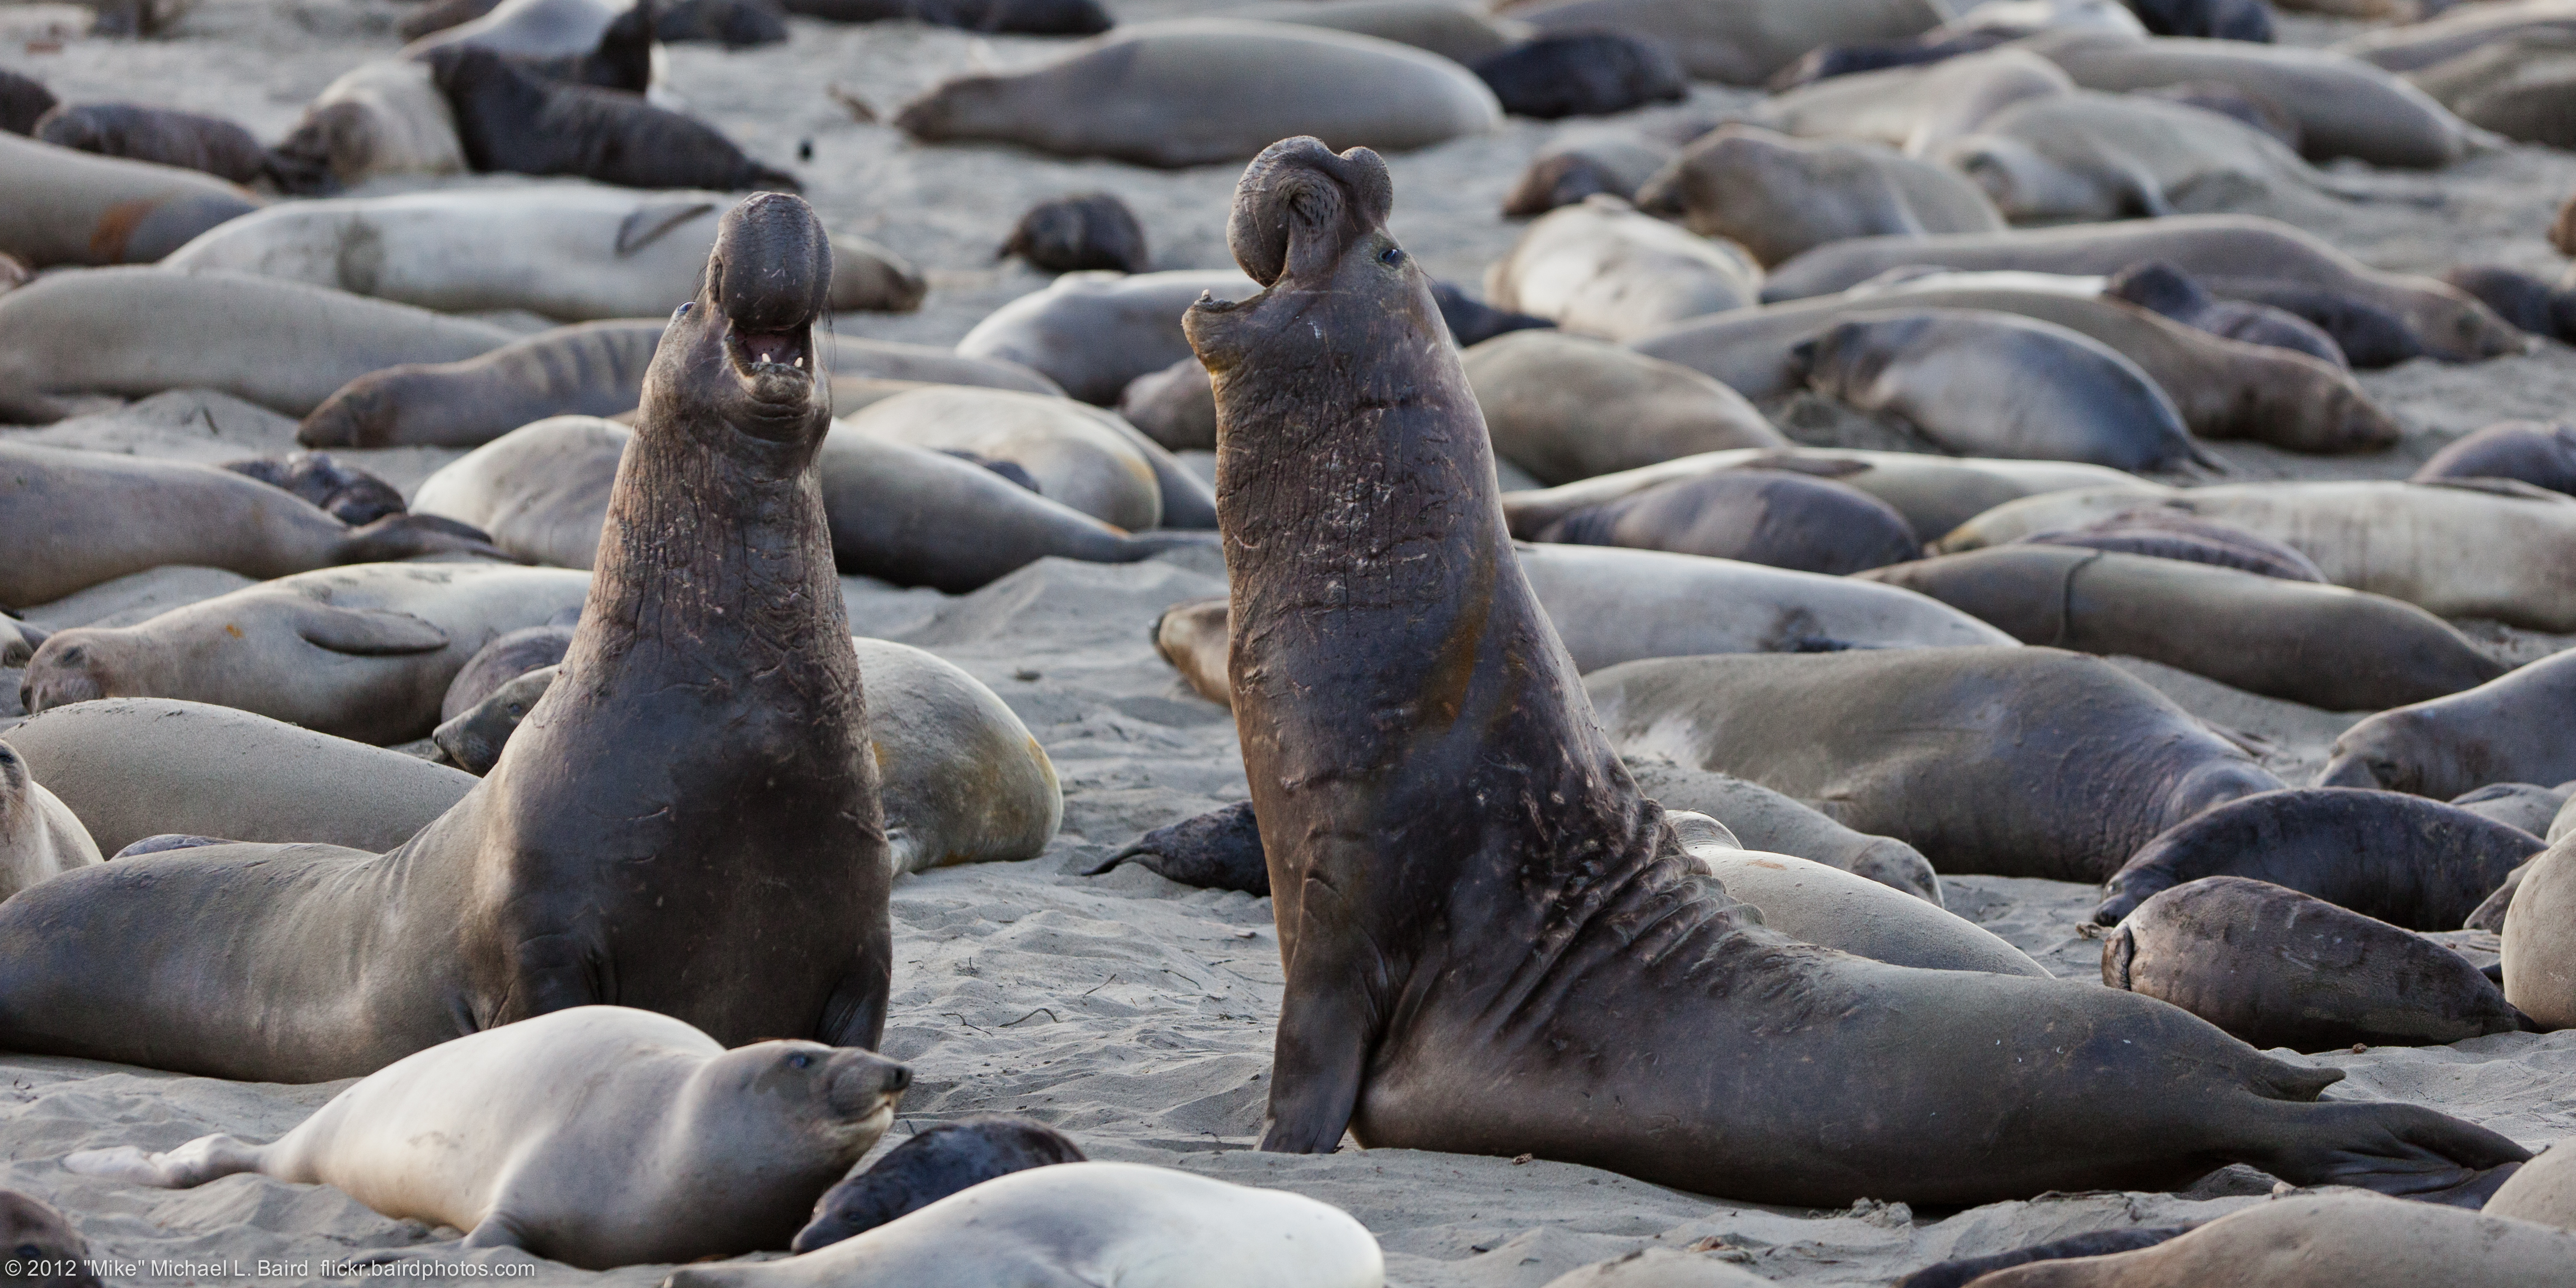
\includegraphics[width=0.55\textwidth]{Pics/elephant_seals} \\
		\caption{Northern elephant seal (\textit{Mirounga angustirostris})}
        \end{figure}

	\small
	Sea elephants were hunted nearly to extintion to a populazione of just 2-20 individuals. Today the population rebounded to 175,000 individuals.

	From historical (before hunting) and modern samples, their genetic diversity* was reduced from 0.90 to 0.41.

	\vskip 0.5cm
	\tiny * (more in this later)

\end{frame}


\begin{frame}{Founder effect}

	\bigskip
	\begin{block}{}
		Reduction in variability caused by a bottleneck in the population size during the founding of a new population.
	\end{block}

	\begin{figure}
                \includegraphics[width=0.65\textwidth]{Pics/founder}
        \end{figure}

\end{frame}


\begin{frame}{Founder effect}

        \begin{figure}
                \includegraphics[width=0.65\textwidth]{Pics/founder}
        \end{figure}

	Genetic divergence after speciation may be helped along by the \textbf{strong} effects of genetic drift in the
	founders of a population.

\end{frame}


\begin{frame}{Intended Learning Outcomes}

	\underline{Genetic drift}

        \bigskip

        In this lecture you have learnt
        \begin{itemize}
                \item to describe the Wright-Fisher model of genetic drift
                \item to calculate expected allele frequencies
                \item to quantify the effect of population size on drift
        \end{itemize}

\end{frame}







\section{Mutation}

\begin{frame}{Intended Learning Outcomes}

	\underline{Mutation}

	\bigskip

	In this lecture you will learn
  	\begin{itemize}
                \item to appreciate the effects of novel mutations on allele frequencies
                \item to describe the concepts of mutation and substitution rate
                \item to calculate divergence times using the molecular clock from genomic data with \texttt{R}
        \end{itemize}

\end{frame}

\begin{frame}{Mutations}

        New mutations arise to produce new genetic variation that genetic drift can act on:
        \begin{itemize}
                \item deletions
                \item insertions
                \item translocations
                \item point mutations
        \end{itemize}

        Any of these mutations can be represented with a di-allelic model (e.g. presence/absence)
        if we assume that multiple mutations cannot occur in the same location*.

	\bigskip
        \tiny * more on this later

\end{frame}


\begin{frame}{Effect of mutations on allele frequency}

	\bigskip

	Assume that the $a$ allele in each individual randomly mutates to $A$ with probability $\mu$ 
	(\textbf{mutation rate}) in each generation.

	\begin{figure}
                \includegraphics[width=0.8\textwidth]{Pics/mutation}
        \end{figure}


\end{frame}

\begin{frame}{Effect of mutations on allele frequency}

        \begin{figure}
                \includegraphics[width=0.6\textwidth]{Pics/mutation}
        \end{figure}

	What is the $E[f_A(t+1)]$ given $f_A(t)$ and $\mu$?
	\pause
	\begin{equation}
		E[f_A(t+1)] = f_A(t) + \mu f_a(t)
	\end{equation}

	\tiny{jupyter-notebook: mutation}

\end{frame}


\begin{frame}{Effect of mutations on allele frequency}

	If mutations occur in both directions, e.g. mutations occur at rate $\mu_{a \rightarrow A}$ from $a$
	to $A$ and $\mu_{A \rightarrow a}$ from $A$ to $a$, then
	\begin{equation}
		E[f_A(t+1)] = (1 - \mu_{A \rightarrow a} ) f_A(t) + \mu_{a \rightarrow A} f_a(t)
	\end{equation}

	\bigskip
	\tiny{jupyter-notebook: mutation}

\end{frame}


\begin{frame}{Effect of mutations on allele frequency}

	In the absence of other forces (e.g. genetic drift and selection), an equilibrium will
	eventually be established:
	\begin{equation}
		f_A = \frac{\mu_{a \rightarrow A}}{\mu_{a \rightarrow A}+\mu_{A \rightarrow a}}
	\end{equation}

\end{frame}


\begin{frame}{Mutation rate}

	\begin{figure}
                \includegraphics[width=0.5\textwidth]{Pics/mutrate}
        \end{figure}

	\small
	\begin{itemize}
		\item mutation is a weak force in higher organisms
		\item with no genetic drift, it takes a long time for the allele frequency to reach equilibrium
		\item we can often ignore recurrent mutations
	\end{itemize}

\end{frame}


\begin{frame}{Probability of fixation}

	The probability that an allele of frequency $1/(2N)$ goes to fixation is $1/(2N)$.

	\bigskip

	\pause
	$Pr(\texttt{fixation of allele A}) = N_A \times (1/2N) = f_A(t) $ at generation $t$.

	\begin{block}{}
	In the absence of selection and mutation, the probability of fixation of an allele is simply its allele frequency.
	It does not depend on the population size.
	\end{block}

\end{frame}


\begin{frame}{Rate of substitution}

	\small
	\begin{block}
	Rate at which mutations accumulate \textbf{between species}. 
	Substitution refers to mutations that have gone to fixation. 
	\end{block}

	\vskip 0.3cm

	Assume:
	\begin{itemize}
		\item mutation rate $\mu$: in each generation $\mu$ new mutations occur in each gene copy (e.g. per site, per gene, ...)
		\item $2N$ gene copies
	\end{itemize}

	\pause

	The expected number of mutations each generation that eventually will go to fixation is
	\begin{equation*}
		2N\mu \times 1/(2N) = \mu
	\end{equation*}
	The rate of substituion is simply the mutation rate.

\end{frame}


\begin{frame}{Molecular clock}

	If
	\begin{itemize}
		\item no selection
		\item "low" mutation rate (not affecting allele frequencies much)
		\item constant mutation rate
	\end{itemize}
	then the rate of substitution should be contant \textit{in time}.

	\bigskip

	\begin{block}{}
		Mutations can be used to date divergence between species.
	\end{block}
	How?

\end{frame}


\begin{frame}{Molecular clock}

	\begin{columns}

        	\column{0.5\textwidth}

                \begin{figure}
                        \includegraphics[width=0.9\textwidth]{Pics/divergence}
                \end{figure}

                \column{0.5\textwidth}
		\small
		The expected number of nucleotide differences separating sequences of the same genes in the two species is $E[d_{AB}] = 2 \mu t_{AB}$.
		
		\bigskip

		Therefore
		\begin{itemize}
			\item $t_{AB}=\frac{2\mu}{d_{AB}}$ or
			\item $\mu = \frac{d_{AB}}{2t_{AB}}$
		\end{itemize}

        \end{columns}

\end{frame}


\begin{frame}{Molecular clock}

	Caveats:
	\begin{itemize}
		\item it depends on an estimate of $\mu$
		\item it assumes no natural selection acting
		\item it assumes that mutation rate is constant and equal among different species
	\end{itemize}

	\bigskip
	Not very realistic but a good approximate for closely related species.

\end{frame}


\begin{frame}{Dating human-chimpanzee divergence time}

	\begin{figure}
        	\includegraphics[width=0.75\textwidth]{Pics/dating}
        \end{figure}

\end{frame}


\begin{frame}{Dating human-chimpanzee divergence time}

	$\mu = 0.07 / (2 \times 25 \times 10^6) = 1.4 \times 10^{-9}$ per site per year

	\bigskip

	$t = 0.012 / (2 \times 1.4 \times 10^{-9}) = 4.3$ million years ago

	\bigskip

	\small

	Compatible but shorted than expected: \\
	generation time as changed and therefore the rate per year changed \\
	effect of natural selection \\
	change in mutation rate \\
	errors in estimating nucleotidic divergence \\
	error in estimating human-macaque divergence time \\
	...
	
\end{frame}


\begin{frame}{Intended Learning Outcomes}

        \underline{Mutation}

	\bigskip

        In this lecture you have learnt
        \begin{itemize}
                \item to appreciate the effects of novel mutations on allele frequencies
                \item to describe the concepts of mutation and substitution rate
                \item to calculate divergence times using the molecular clock from genomic data with \texttt{R}
        \end{itemize}

\end{frame}





\section{Coalescence theory}

\begin{frame}{Intended Learning Outcomes}

        \underline{Coalescence theory}

	\bigskip

        In this lecture you will learn to
	\begin{itemize}
                \item describe principles and assumptions of the coalescence theory
                \item discuss the infinite sites model
                \item provide estimators of $\theta$ and effective population size
                \item measure genetic variability with summary statistics and the site frequency 
		spectrum with \texttt{R}
        \end{itemize}

\end{frame}


\begin{frame}{Motivation}

	\begin{figure}
                \includegraphics[width=0.7\textwidth]{Pics/data_theory}
        \end{figure}

\end{frame}


\begin{frame}{Motivation}

	e.g. on the X chromosomes, two Europeans differ, on average, in $0.08\%$ of sites, while
	individuals from African populations differ in $0.012\%$ of sites.

	\bigskip

	What do these numbers tell us \textit{about} the two populations?

	\pause

	\begin{block}{}
	We use \textbf{coalescence theory}, which is based on Wright-Fisher model, to consider the genealogy history
	of a sample and make inferences about populations instead of modelling changes of allele frequencies forward in time.
	\end{block}


\end{frame}


\begin{frame}{Coalescence}

	\begin{figure}
                \includegraphics[width=0.5\textwidth]{Pics/coalescence} \
		\caption{Tracking the ancestry of a sample between two generations.}
        \end{figure}

\end{frame}


\begin{frame}{Coalescence}

	If two individual gene copies have the same parent in the previous generation, we say that the \textbf{ancestral lineage}
	representing these two individuals have \textbf{coalesced}.

	\bigskip

	They have a \textbf{common ancestor} and a \textbf{coalescent event} has occured.

\end{frame}


\begin{frame}{Coalescence tree}

        \begin{figure}
                \includegraphics[width=0.7\textwidth]{Pics/coal_tree} \
                \caption{Ancestry of three samples.}
        \end{figure}

\end{frame}


\begin{frame}{Coalescence tree}

	The ancestry of an individual gene copy is represented by a line (or edge).

	\bigskip
	\begin{block}{}
	The time until two lineages find a \textbf{most recent common ancestor (MRCA)} is called \textbf{coalescence time}.
	\end{block}

	How can we find the coalescence time?

\end{frame}


\begin{frame}{Coalescence in a sample of two gene copies}

	As there are $2N$ potential parents "chosen" with equal probability, the probability of two individuals having the same
	parent in the previous generation is \pause $1/(2N)$.

	\bigskip

	The probability that two gene copies did NOT have the same parent in the previous generation is \pause $1-1/(2N)$.

	\bigskip

	The probability that two gene copies did not have the same parent in the past $r$ generations is \pause $[1-1/(2N)]^r$.

\end{frame}


\begin{frame}{Coalescence in a sample of two gene copies}

	The probability of not finding any common ancestor in generation $r-1$ but then finding the first common ancestor
	in generation $r$ is \pause
	\begin{equation}
		Pr(\texttt{...}) = [1-1/(2N)]^{r-1}[1/(2N)]
	\end{equation}

	\small

	This equation gives us the probability distribution of the time to the MRCA in a sample if size $n=2$. This is 
	a geometric random variable: the probability distribution of the number of Bernoulli trials needed to get one success.

	\bigskip
	\tiny
	jupyter-notebook: coalescence

\end{frame}


\begin{frame}{Coalescence in large populations}

	\begin{itemize}
		\item If we consider the limit of an infinitely large population, calculations 
		simplify but we can still 
		consider the effect of genetic drift.
		\item It is convenient to measure time in $2N$ generations, by setting $r=2Nt$ with $t$ measuring time in $2N$ generations.
	\end{itemize}

	\pause
	The probability that two gene copies do not find a common ancestor in $2Nt$ generations becomes
	\begin{equation*}
		[1-1/(2N)]^{2Nt} \rightarrow e^{-t} \texttt{ as } N \rightarrow \infty
	\end{equation*}


\end{frame}


\begin{frame}{Coalescence in large populations}

	As $N$ becomes large, the distribution of the coalescence times follows an \textbf{exponential distribution} with mean 1.

	\bigskip

	As time is measured in $2N$ generations, the mean (expected) time to coalescence is actually $2N$ generations.
	In other words, there is a constant rate of coalescence of $1$ per $2N$ generations.
	
	\bigskip
	\tiny
        jupyter-notebook: coalescence

\end{frame}


\begin{frame}{Coalescence in large population}

	\begin{itemize}
		\item The random process of following the lineages backward in time until a most recent common ancestor
		has been found is called a \textbf{coalescence process}.
		\item It is intuitive to understand that the expected coalescence time is $2N$ generations, although
		there is considerable variability in the coalescence times.
	\end{itemize}

\end{frame}


\begin{frame}{Coalescence in large population}

        \begin{itemize}
		\item The coalescence process in a large randomly mating diploid population with two sexes is the same as that
		in the simple haploid model.
		\item Once we have a conveniente description of the geneaology, then it is easy to derive various properties
		of our sample.
	\end{itemize}

\end{frame}


\begin{frame}{Genetic variability and population size}

	\begin{columns}

                \column{0.4\textwidth}

                \begin{figure}
                        \includegraphics[width=0.9\textwidth]{Pics/tau}
                \end{figure}

                \column{0.6\textwidth}
          

		We expect $2N\mu t$ mutations on a lineage of length $t$. 

		Since $E[t]=1$ and there are two lineages,
		the expected number of mutations separating two gene copies is
		\begin{equation}
			\theta = 4N\mu
		\end{equation}
		which is a simple relationship between the amount of genetic variability and population sizes.

        \end{columns}

\end{frame}


\begin{frame}{Genetic variability and population size}

        \begin{columns}

                \column{0.4\textwidth}

                \begin{figure}
                        \includegraphics[width=0.9\textwidth]{Pics/tau}
                \end{figure}

                \column{0.6\textwidth}
 
		The expected number of mutations occuring in a lineage during any time interval of length $\tau$ is 
		$2N\mu\tau=\tau \theta /2$.

		\bigskip
		\small

		As such, we can think of the data generated by a coalescence process producing a coalescence tree and a 
		subsequent process in which mutations are distributed across the lineage of the tree at rate $\theta /2$.

        \end{columns}

\end{frame}


\begin{frame}{Infinite Sites Model}

	\begin{block}{}
		Each new mutation creates a new variable site, i.e. that each new mutation hits a new site in the sequence, such that no site experiences more than one mutation.
	\end{block}

	\bigskip

	\begin{figure}
        	\includegraphics[width=0.9\textwidth]{Pics/iam} \\
		\caption{\small The sequence is infinitely long so that the chance of two mutations hit the same site is essentially zero.}
        \end{figure}

\end{frame}


\begin{frame}{Infinite Sites Model}

	The sites in which some of the individuals differ are called
	\textbf{segregating sites} or \textbf{single nucleotide polymorphisms} (SNPs).

 	\begin{figure}
                \includegraphics[width=0.7\textwidth]{Pics/sequences} 
        \end{figure}

	Under the infinite sites model, we can deduce which mutations occurred
	in the ancestry of a sample of sequences.

\end{frame}


\begin{frame}{Infinite Sites Model}

	The model does not distinguish between different nucleotides and does
        not care about invariable sites.

	\begin{figure}
                \includegraphics[width=0.5\textwidth]{Pics/sequences01} \\
		\caption{\small Data as a binary matrix of the variable sites.}
        \end{figure}

\end{frame}


\begin{frame}{Infinite Sites Model}

	\begin{itemize}
		\item Labelling with zeros and ones is arbitrary.
		\item Good approximation if the rate of mutation is low.
		\item DNA sequences with different mutations are different \textbf{haplotypes}.
	\end{itemize}

	\begin{figure}
                \includegraphics[width=0.1\textwidth]{Pics/sequences01_only} \\
		\caption{How many DNA sequences? How many haplotypes?}
        \end{figure}

\end{frame}


\begin{frame}{Tajima's estimator}

	We want an estimate of $\theta=4N\mu$ under the infinite sites model from the expected number of
	mutations separating two individuals based on the DNA sequences obtained from data.

	\pause
	\bigskip

	Data can be summarised as the \textbf{average number of pairwise differences}, or $\pi$.
	\begin{equation}
		\pi = \frac{\sum_{i<j}d_{i,j}}{n(n-1)/2}
	\end{equation}
	with $n$ sequences, $d_{i,j}$ number of differences between sequence $i$ and $j$.

\end{frame}


\begin{frame}{Tajima's estimator}

	\begin{figure}
                \includegraphics[width=0.1\textwidth]{Pics/sequences01_only} \\
		\caption{What is the value of $\pi$?}
        \end{figure}

	\pause
	$\pi = (2+2+2+2+0+2+2+2+2+0)/(5x4/2)=1.6$

\end{frame}


\begin{frame}{Tajima's estimator}

	\begin{columns}

                \column{0.3\textwidth}

                \begin{figure}
                        \includegraphics[width=0.9\textwidth]{Pics/tau}
                \end{figure}

                \column{0.7\textwidth}

		The expected number of nucleotide differences between two sequences is the expected 
		number of mutations, $\theta=4N\mu$.

		\begin{equation}
			E[d_{i,j}] = \theta
		\end{equation}

		\begin{equation}
			E[\pi] = \theta
		\end{equation}

		$\hat{\theta}_T = \pi$ is called \textbf{Tajima's} estimator of $\theta$.

        \end{columns}

\end{frame}


\begin{frame}{Effective population size}

	\begin{block}{}
		The number of individuals in a Wright-Fisher model that would produce the same amount of
		genetic drift as in the real population.
	\end{block}

	The amount of genetic drift can be measured as
	\begin{itemize}
		\item the expected heterozygosity
		\item expected number of pairwise differences
		\item rate of coalescence
		\item ...
	\end{itemize}

\end{frame}


\begin{frame}{Effective population size ($N_e$)}

	\textit{e.g. "A population with an effective size of 200 with respect to heterozygosity harbours
	the same amount of heterozygosity as a Wright-Fisher population of 200 individuals."}

	\bigskip

	The true number of individuals in the population can be very different from its effective
	population size!

\end{frame}


\begin{frame}{Effective population size}

	\begin{figure}
        	\includegraphics[width=0.7\textwidth]{Pics/salmon} \\
		\caption{The effective population size of the Chinook salmon (\textit{Oncorhynchus tshawytscha}) 
	  	has been estimated to be very low, possibly because the population size fluctuates between years and high variance
	  	offspring.} 
        \end{figure}

\end{frame}


\begin{frame}{Effective population size ($N_e$)}

	\begin{figure}
                \includegraphics[width=0.4\textwidth]{Pics/ne_change}
	\end{figure}

	\small

	If a population fluctuates between sizes $N_1$, $N_2$, ..., $N_k$ at a proportion $p_1$, $p_2$, ..., $p_k$
	of the time, the coalescent effective population size is the harmonic mean:
	\begin{equation}
		N_e = \frac{1}{p_1/N_1 + p_2/N_2 + ... p_k/N_k}
	\end{equation}
	which is smaller that the arithmetic mean and gives more weight to smaller sizes.


\end{frame}


\begin{frame}{Effective population size ($N_e$)}

	\begin{figure}
                \includegraphics[width=0.4\textwidth]{Pics/chickens}
        \end{figure}

	The effective population size with unequal sex ratio is
	\begin{equation}
		N_e = \frac{4N_mN_f}{N_m+N_f}
	\end{equation}
	which is smaller than $N_m+N_f$.

\end{frame}


\begin{frame}{Interpreting estimates of $\theta$}

	\begin{table}[h]
                \centering
                \begin{tabular}{p{0.2\textwidth} p{0.7\textwidth}}
                        \toprule
                        \multicolumn{2}{p{0.9\textwidth}}{$\pi$ on autosomes} \\
                        \midrule
                        Mandenka    & 0.00120 \\
                        Biaka       & 0.00121 \\
			San & 0.00126 \\
                        Han & 0.00081 \\
			Basque & 0.00087 \\
			Melanesians & 0.00078 \\
                        \bottomrule
                \end{tabular}
        \end{table}

\end{frame}


\begin{frame}{Interpreting estimates of $\theta$}

        \begin{table}[h]
                \centering
                \begin{tabular}{p{0.2\textwidth} p{0.7\textwidth}}
                        \toprule
                        \multicolumn{2}{p{0.9\textwidth}}{$\pi$ on X chromosomes} \\
                        \midrule
                        Mandenka    & 0.00099 \\
                        Biaka       & 0.00095 \\
                        San & 0.00085 \\
                        Han & 0.00058 \\
                        Basque & 0.00071 \\
                        Melanesians & 0.00066 \\
                        \bottomrule
                \end{tabular}
        \end{table}

\end{frame}


\begin{frame}{Watterson's estimator}

	\begin{equation}
		\hat{\theta}_W = \frac{S}{\sum_{k=1}^{n-1} \frac{1}{k}}
	\end{equation}
	with $S$ segregating sites and $n$ samples.

	\begin{equation}
		E[\hat{\theta}_W] = \theta
	\end{equation}

\end{frame}


\begin{frame}{Watterson's estimator}

        \begin{figure}
                \includegraphics[width=0.1\textwidth]{Pics/sequences01_only} \\
                \caption{What is the value of $\hat{\theta}_W$?}
        \end{figure}

        \pause
        $\hat{\theta}_W = 3 / (1+1/2+1/3+1/4)=1.4$ \\
	but before we obtained $\hat{\theta}_T=1.6$. \\
	Why?
	
\end{frame}


\begin{frame}{Summary statistics}

	Possible summaries of DNA sequence data are:
	\begin{itemize}
		\item the number of segregating sites ($S$)
		\item the average number of pairwise differences ($\pi$)
	\end{itemize}
	but they don't provide much information regarding \textbf{allele frequencies}.

\end{frame}


\begin{frame}{The Site Frequency Spectrum (SFS)}

	\begin{block}{SFS}
	The SFS is obtained by tabulating the sample allele frequencies of all mutations.
	\end{block}

	\begin{columns}

                \column{0.2\textwidth}

                \begin{figure}
                        \includegraphics[width=0.6\textwidth]{Pics/sequences01_only}
                \end{figure}

                \column{0.8\textwidth}

		\pause

		The "1" alleles have frequencies $2/5$, $2/5$ and $4/5$.

		The proportions of "1" alleles with a frequency of $1/5$, $2/5$, $3/5$ and $4/5$
		in the sample are \pause $f_1=0$, $f_2=2/3$, $f_3=0$ and $f_4=1/3$.

                \begin{equation*}
                        \vec{f} = (f_1, f_2, ..., f_{n-1})
                \end{equation*}
		for a sample of $n$ haploid individuals.

        \end{columns}

\end{frame}


\begin{frame}{The Site Frequency Spectrum (SFS)}

        \begin{columns}

                \column{0.2\textwidth}

                \begin{figure}
                        \includegraphics[width=0.6\textwidth]{Pics/sequences01_only}
                \end{figure}

                \column{0.8\textwidth}

		\begin{figure}
                        \includegraphics[width=0.75\textwidth]{Pics/SFS}
                \end{figure}

        \end{columns}

\end{frame}


\begin{frame}{Alleles}

	\small
	\begin{itemize}
		\item \textbf{ancestral} allele is the allele found in the MRCA of the sample.
		\item \textbf{derived} allele (or mutated) is an allele that is not ancestral.
	\end{itemize}

	\begin{figure}
        	\includegraphics[width=0.8\textwidth]{Pics/ancder}
        \end{figure}

\end{frame}


\begin{frame}{Alleles}

	\bigskip
	\small
	The ancestral allele is often inferred using \textbf{outgroups}.
	
	e.g. if $C/T$ polymorphism in humans and primate have $C$, then $C$ is likely to be the ancestral allele.

	\begin{figure}
                \includegraphics[width=0.5\textwidth]{Pics/ancder_species}
        \end{figure}

\end{frame}


\begin{frame}{Alleles}

        \begin{figure}
                \includegraphics[width=0.9\textwidth]{Pics/ancder_unknown}
        \end{figure}

\end{frame}


\begin{frame}{The Site Frequency Spectrum (SFS)}

	If no information on the ancestral allele is available, we can \textit{fold} the frequency
	spectrum.
	\begin{block}{}
	The \textbf{folded frequency spectrum} $f^*$ is obtained by adding together the frequencies
	of the derived and ancestral alleles.
	\end{block}

	$f^* = f_i + f_{n-j}$ for $j<n/2$ and \\
	$f^* = f_j$ for $j=n/2$ \\
	only defined for values of $f^* \leq n/2$.

\end{frame}


\begin{frame}{The folded SFS}

        \begin{columns}

                \column{0.2\textwidth}

                \begin{figure}
                        \includegraphics[width=0.6\textwidth]{Pics/sequences01_only}
                \end{figure}

                \column{0.8\textwidth}

		$\vec{f^*} = $ \pause $(f^*_1=1/3, f^*_2=2/3)$

        \end{columns}

\end{frame}


\begin{frame}{The Site Frequency Spectrum}

	\begin{itemize}
		\item $S$ and $\pi$ can be calculated directly from $\vec{f}$ but the opposite is not true.
		\item Alleles segregating at frequency of $1/n$ are called \textbf{singletons}.
		\item The expected SFS under the standard coalescence model with infinite sites mutations is
		\begin{equation}
			E[f_i] = \frac{1/j}{\sum_{k=1}^{n-1} \frac{1}{k}}
		\end{equation}
		with $j=1,2,...,n-1$
	\end{itemize}

	\bigskip
	\tiny jupyter-notebook: coalescence

\end{frame}


\begin{frame}{Tree shape and population size}

	\small
	Measured in number of generations, the expected coalescence time for $k$ lineages is $2N/[k(k-1)]$.

	\begin{figure}
         	\includegraphics[width=0.85\textwidth]{Pics/tree_N_i}
        \end{figure}

\end{frame}


\begin{frame}{Tree shape and population size}

        \small
        Measured in number of generations, the expected coalescence time for $k$ lineages is $2N/[k(k-1)]$.

        \begin{figure}
                \includegraphics[width=0.85\textwidth]{Pics/tree_N_d}
        \end{figure}

\end{frame}


\begin{frame}{Intended Learning Outcomes}

        \underline{Coalescence theory}

        \bigskip

        In this lecture you have learnt to
        \begin{itemize}
                \item describe principles and assumptions of the coalescence theory
                \item discuss the infinite sites model
                \item provide estimators of $\theta$ and effective population sizes
		\item measure genetic variability with summary statistics and the site 
		frequency spectrum with \texttt{R}
        \end{itemize}

\end{frame}












\section{Population subdivision}

\begin{frame}{Intended Learning Outcomes}

	\underline{Population subdivision}

	\bigskip

	In this lecture you will learn to
	\begin{itemize}
		\item quantify the effect of population subdivision on allele frequencies and heterozygosity
		\item calculate measures of population genetic differentiation
		\item discuss divergence models
	\end{itemize}

\end{frame}


\begin{frame}{Population subdivision}

	\begin{block}{}
		There is population subdivision, or \textbf{structure}, when the population is not randomly mating
		because of geographic or social structure.
	\end{block}

	\bigskip

	Population subdivision is important to
	\begin{itemize}
		\item understand the effects of drift and natural selection
		\item plan conservation strategies for rare or endangered species
	\end{itemize}

\end{frame}


\begin{frame}{Population subdivision}

        \begin{figure}
                \includegraphics[width=0.65\textwidth]{Pics/predivision}
        \end{figure}

\end{frame}


\begin{frame}{Population subdivision}

	\begin{figure}
                \includegraphics[width=0.65\textwidth]{Pics/division}
        \end{figure}

\end{frame}


\begin{frame}{Allele frequencies in a subdivided population}

        \begin{columns}

                \column{0.3\textwidth}

                \begin{figure}
			\includegraphics[width=0.8\textwidth]{Pics/predivision} \
                        \includegraphics[width=0.8\textwidth]{Pics/division}
                \end{figure}

                \column{0.7\textwidth}

		Assume two subpopulations, each one in HW equilibrium with $N_1$ and $N_2$ individuals, respectively.

		\vskip 0.5cm

		The average frequency of allele $A$ when pooling the two subpopulations is
		\begin{equation}
			f_A = \frac{2 N_1 f_{A1} + 2 N_2 f_{A2}}{2N_1 + 2N_2}
		\end{equation}
		If $N_1=N_2$
		\begin{equation}
                        f_A = \frac{f_{A1} + f_{A2}}{2}
                \end{equation}

        \end{columns}

\end{frame}


\begin{frame}{Heterozygosity in a subdivided population}

        \begin{columns}

                \column{0.3\textwidth}

                \begin{figure}
			\includegraphics[width=0.8\textwidth]{Pics/predivision} \
                        \includegraphics[width=0.8\textwidth]{Pics/division}
                \end{figure}

                \column{0.7\textwidth}

		The proportion of heterozygous individuals is
                \begin{equation}
                        H_S = \frac{2f_{A1}(1-f_{A1}) + 2f_{A2}(1-f_{A2})}{2}
                \end{equation}
		which is the expected heterozygosity when both populations are sampled.

		\bigskip

		\small{$S$ in $H_S$ stands for "in the \underline{s}ubdivided population"}
	
        \end{columns}

\end{frame}


\begin{frame}{Heterozygosity in a subdivided population}

        \begin{columns}

                \column{0.3\textwidth}

                \begin{figure}
			\includegraphics[width=0.8\textwidth]{Pics/predivision} \
                        \includegraphics[width=0.8\textwidth]{Pics/division}
                \end{figure}

                \column{0.7\textwidth}

                However, the expected proportion of heterozygous individuals in a population with frequency $f_A$ is
                \begin{equation}
                        H_T = 2 \frac{f_{A1} + f_{A2}}{2} (1 - \frac{f_{A1} + f_{A2}}{2})
                \end{equation}

                \bigskip

                \small{$T$ in $H_T$ stands for "in the \underline{t}otal (pooled) population"}
        
        \end{columns}

\end{frame}


\begin{frame}{Heterozygosity in a subdivided population}

	After some rearrangements we have
	\begin{equation}
		H_S = f_{A1}(1-f_{A1}) + f_{A2}(1-f_{A2})
	\end{equation}
	and
	\begin{equation}
                H_T = f_{A1}(1-f_{A1}) + f_{A2}(1-f_{A2}) + \delta^2/2
        \end{equation}
	with $\delta = |f_{A1}-f_{A2}|$.

\end{frame}


\begin{frame}{Heterozygosity in a subdivided population}

	$H_T = H_S + \delta^2/2$

	\begin{itemize}
		\item If $\delta=0$ then \pause $H_T=H_S$ and the total (pooled) population is also in HWE.
		\item If $\delta>0$ then \pause $H_T<H_S$ and \pause the total (pooled) population contains fewer 
		heterozygous individuals than expected given the pooled allele frequency.
	\end{itemize}

	\begin{block}{Wahlund effect}
		The decrease of heterozygosity in a subdivided population compared to a randomly
		mating one with the same (total) allele frequency.
	\end{block}

\end{frame}


\begin{frame}{Quantifying population subdivision}

	\begin{equation}
		F_{ST} = \frac{H_T - H_S}{H_T}
	\end{equation}

	\pause
	$F_{ST}$ has a range defined as
	\begin{itemize}
		\item if $\delta=0$ then $H_T=H_S$ and $F_{ST}=0$
		\item if $\delta=1$ then $F_{ST}=1$
	\end{itemize}

	\bigskip

	$F_{ST}$ can be calculated for more than two subpopulations.

\end{frame}


\begin{frame}{$F_{ST}$: population genetic differentiation}

	\begin{figure}
        	\includegraphics[width=0.5\textwidth]{Pics/whale} \
		\caption{\small Humpback whales in the Pacific and Atlantic have strong genetic differentiation ($F_{ST}>0.4$) while populations in the North Atlantic have low differentation  ($F_{ST} \approx 0.04$).}
        \end{figure}

\end{frame}


\begin{frame}{Wright-Fisher model with migration}

        \begin{figure}
                \includegraphics[width=0.6\textwidth]{Pics/migration} \
                \caption{\small An individual from one population is replaced with an individual from the other with probability $m$ (migration rate).}
        \end{figure}

\end{frame}


\begin{frame}{$F_{ST}$ and migration rates}

	Using the coalescence theory assuming an infinite sites model, we can derive that
	\begin{equation}
		F_{ST} = \frac{1}{1 + 4Nm_T}
	\end{equation}
	with $m_T$ being the total number of migrants.

	\bigskip
	\tiny jupyter-notebook: subdivision

\end{frame}


\begin{frame}{"Island" model}

	\small
	\begin{block}{}
	It assumes that populations have been subdivided for a very long time so that 
	an equilibrium has been established and that then there is ongoing \textbf{gene-flow}.
	\end{block}
	It is not a realistic model for some species.

	\pause
	\begin{figure}
                \includegraphics[width=0.6\textwidth]{Pics/human_evo}
        \end{figure}


\end{frame}


\begin{frame}{Divergence model}

	\small
	\begin{block}{}
		It describes populations diverging from common ancestral populations without subsequent gene-flow.
	\end{block}

	\begin{figure}
                \includegraphics[width=0.3\textwidth]{Pics/coal_divergence} \
		\caption{\small TMRCA overestimates the divergence time.}
        \end{figure}

\end{frame}


\begin{frame}{Isolation by distance}

	\begin{block}{}
		The degree of population subdivision increases with geographical distance.
	\end{block}

	\bigskip

	\begin{itemize}
		\item migration rate is a linear function of geographical distance
		\item migration occurs only between adjacent populations (stepping-stone models)
		\item series of divergence events (sequential colonisation)
	\end{itemize}

\end{frame}

\begin{frame}{Isolation by distance}

	\begin{figure}
                \includegraphics[width=0.9\textwidth]{Pics/handley} \
                \caption{\small Isolation by distance in human populations.}
        \end{figure}

\end{frame}


\begin{frame}{Intended Learning Outcomes}

        \underline{Population subdivision}

        \bigskip

        In this lecture you have learned to
        \begin{itemize}
                \item quantify the effect of population subdivision on allele frequencies and heterozygosity
                \item calculate measures of population genetic differentiation
                \item discuss divergence models
        \end{itemize}

\end{frame}





\section{Demographic inference}


\begin{frame}{Intended Learning Outcomes}

	\underline{Demographic inference}

	Through examples from the literature, in this lecture you will learn to
	\begin{itemize}
		\item make inferences on population history from genomic data with \texttt{R}
		\item interpret results from population genetics studies
		\item design a genomic study
		\item (discuss the effect of demography on signatures of natural selection)
	\end{itemize}

\end{frame}




\begin{frame}{!}

	Please do not redistribute. Some material may be protected by copyright.

\end{frame}

 
\end{document}

